\documentclass[10pt,conference,twocolumn]{IEEEtran}
\IEEEoverridecommandlockouts
\usepackage{cite}
\usepackage{amsmath,amssymb,amsfonts}
\usepackage{algorithmic}
\usepackage{graphicx}
\usepackage{textcomp}
\usepackage{xcolor}
\usepackage{booktabs}
\usepackage{multirow}
\usepackage{stfloats}
\usepackage{hyperref}

\hypersetup{
    colorlinks=true,
    linkcolor=blue,
    citecolor=blue,
    urlcolor=blue
}

\def\BibTeX{{\rm B\kern-.05em{\sc i\kern-.025em b}\kern-.08em
    T\kern-.1667em\lower.7ex\hbox{E}\kern-.125emX}}

\begin{document}

\title{Validade Temporal e Supersessão de Fatos em Memória Associativa Hebbiana para Agentes Baseados em LLM\\
\large Relatório Técnico de Replicação Experimental e Proposta Arquitetural}

\author{\IEEEauthorblockN{Filipe Augusto de Ataíde Barbosa}
\IEEEauthorblockA{\textit{Centro de Informática (CIn)} \\
\textit{Universidade Federal de Pernambuco (UFPE)}\\
Recife, Brasil \\
faab@cin.ufpe.br / filipeataide@gmail.com}
}

\maketitle

\begin{abstract}
Agentes conversacionais autônomos baseados em Grandes Modelos de Linguagem (LLMs) requerem memórias de longo prazo capazes de sintetizar informações dispersas e manter consistência factual contínua. Arquiteturas recentes fundamentadas em plasticidade sináptica hebbiana, notadamente o framework \textit{HeLa-Mem} (ACL 2026), demonstraram notável eficiência na recuperação associativa de múltiplos saltos (\textit{multi-hop retrieval}). Contudo, uma investigação aprofundada revela uma lacuna epistemológica nesses sistemas: a fusão indiscriminada entre o momento de registro de uma memória e o período efetivo de validade do fato subjacente. Sem modelagem de supersessão temporal, fatos obsoletos competem diretamente com estados correntes, gerando anacronismos e respostas alucinadas. Este trabalho estabelece o fundamento experimental para sanar essa limitação. Inicialmente, realiza-se uma replicação empírica estrita da baseline do \textit{HeLa-Mem} sobre a totalidade do benchmark \textit{LongMemEval-S} (500 instâncias de teste), obtendo 61,20\% de acurácia global (frente a 65,40\% da meta oficial), com superação em \textit{Temporal Reasoning} (51,88\% vs. 50,38\%) e em \textit{Single-Session User} (87,14\% vs. 78,85\%). A análise de erros demonstra que 43,8\% de todas as falhas da baseline concentram-se precisamente em raciocínio temporal e atualização de conhecimento. Com base nesse diagnóstico, formaliza-se a \textbf{Solução Proposta}: uma extensão à memória semântica que modela janelas de validade temporal $[t_{start}, t_{end}]$, arestas explícitas de supersessão e uma função de recuperação ponderada pela data da consulta ($t_{query}$). O documento apresenta quatro figuras em resolução de publicação detalhando o contraste arquitetural, a anatomia das falhas e um estudo de caso qualitativo, consolidando a baseline oficial congelada para a avaliação comparativa subsequente.
\end{abstract}

\begin{IEEEkeywords}
Memória para Agentes, Plasticidade Hebbiana, Validade Temporal, Supersessão Factual, LongMemEval-S, Deep Learning.
\end{IEEEkeywords}

% =========================================================================
% SEÇÃO I: SOLUÇÃO PROPOSTA
% =========================================================================
\section{Solução Proposta}

\subsection{A Tensão entre Plasticidade Associativa e Validade Epistêmica}
A persistência de memória em agentes interativos enfrenta um dilema fundamental entre conectividade associativa e precisão temporal. Modelos de grafos associativos com aprendizado hebbiano~\cite{helamem2026} fortalecem conexões sinápticas entre nós coativados (\textit{``neurons that fire together, wire together''}), o que viabiliza a recuperação contextualmente rica de informações correlatas. No entanto, o princípio hebbiano captura puramente coocorrência e afinidade semântica, permanecendo agnóstico quanto à veracidade cronológica dos fatos no instante da consulta.

No pipeline do HeLa-Mem, os nós da Memória Semântica (\texttt{HebbianKnowledgeMemory}) armazenam proposições extraídas de forma estática com metadados elementares (\texttt{\{"type": "fact"\}}). O decaimento temporal implementado ($\gamma = e^{-\Delta t / \tau}$) é restrito ao momento de execução do código em runtime, calculando o intervalo decorrido em relação ao relógio local da máquina e não em relação à linha do tempo intrínseca da conversa. Consequentemente, quando um fato é revogado (por exemplo, a mudança de residência ou cargo de um usuário), o fato ancestral e o fato sucessor coexistem indefinidamente no grafo com pesos positivos. Durante a consulta, o motor vetorial recupera ambos com escores similares, transferindo ao modelo gerador o ônus de desambiguar contradições históricas em sua janela de contexto.

\subsection{Formalização do Grafo de Conhecimento Temporal}
Para equacionar essa limitação sem desestruturar a dinâmica hebbiana do grafo episódico, propõe-se uma representação de memória semântica consciente de tempo, inspirada nos princípios temporais do Zep/Graphiti~\cite{zep2025}. 

Define-se o grafo de conhecimento temporal como $\mathcal{G}_{temp} = (\mathcal{F}, \mathcal{E}_{heb}, \mathcal{E}_{sup})$, onde $\mathcal{F}$ denota o conjunto de fatos, $\mathcal{E}_{heb}$ o conjunto de arestas hebbianas ponderadas por força sináptica $w_{ij}$, e $\mathcal{E}_{sup}$ o conjunto de arestas direcionadas de supersessão. Cada fato consolidado $f_i \in \mathcal{F}$ é formalizado como uma 5-upla:
\begin{equation}
f_i = \langle c_i, \mathbf{e}_i, [t_{start}^{(i)}, t_{end}^{(i)}], \mathcal{S}_i, \mathbf{w}_i \rangle
\end{equation}
onde:
\begin{itemize}
    \item $c_i$: proposição textual do fato consolidado;
    \item $\mathbf{e}_i \in \mathbb{R}^d$: embedding vetorial denso de $c_i$;
    \item $[t_{start}^{(i)}, t_{end}^{(i)}]$: intervalo fechado à esquerda de validade temporal do fato, extraído diretamente dos metadados temporais originais da sessão (\texttt{haystack\_dates});
    \item $\mathcal{S}_i \in \mathcal{F} \cup \{\emptyset\}$: ponteiro explícito de supersessão (\textit{superseded\_by}), apontando para o fato $f_j$ que revogou $f_i$;
    \item $\mathbf{w}_i$: vetor de acoplamento hebbiano com os demais nós em $\mathcal{F}$.
\end{itemize}

\subsection{Mecanismo de Supersessão e Atualização Incremental}
A atualização da memória semântica ocorre dinamicamente a cada sessão $S_k$ ocorrida no instante $t_{event}$. Ao extrair um novo fato candidato $f_{new}$, o sistema realiza uma varredura semântica sobre o subconjunto de fatos vigentes $\mathcal{F}_{active} = \{f \in \mathcal{F} \mid t_{end} = \infty\}$ calculando a similaridade de cosseno $\text{Sim}(\mathbf{e}_{cand}, \mathbf{e}_{new})$. Para candidatos com similaridade superior ao limiar $\theta_{sem}$, um classificador estruturado determina a transição relacional:
\begin{enumerate}
    \item \textbf{UNRELATED}: os fatos abordam entidades ou propriedades ortogonais; ambos permanecem ativos em $\mathcal{F}_{active}$.
    \item \textbf{EXTENDS}: $f_{new}$ agrega nuances complementares a $f_{cand}$. Mantém-se $t_{end}^{(cand)} = \infty$ e incrementa-se a aresta hebbiana $w(f_{cand}, f_{new}) \leftarrow w(f_{cand}, f_{new}) + \eta$.
    \item \textbf{SUPERSEDES}: $f_{new}$ refuta, substitui ou atualiza o estado afirmado por $f_{cand}$. Aplica-se a transição atômica:
    \begin{align}
        t_{end}^{(cand)} &\leftarrow t_{event} \\
        \mathcal{S}_{cand} &\leftarrow f_{new} \\
        (f_{cand}, f_{new}) &\in \mathcal{E}_{sup} \\
        t_{start}^{(new)} &\leftarrow t_{event}, \quad t_{end}^{(new)} \leftarrow \infty
    \end{align}
\end{enumerate}

Essa modelagem impede o esquecimento catastrófico: o fato $f_{cand}$ permanece preservado para consultas retrospectivas (ex.: ``onde o usuário morava no ano anterior?''), mas tem sua validade terminada no instante $t_{event}$, impedindo sua interferência em consultas sobre o estado presente.

\subsection{Recuperação Ponderada por Pertinência Temporal}
O benchmark LongMemEval disponibiliza o instante exato da pergunta ($t_{query}$). Enquanto a baseline original ignora essa variável na fase de busca em grafo, a solução proposta formula uma função contínua de pertinência temporal $\mathcal{V}(f_i, t_{query})$:
\begin{equation}
\mathcal{V}(f_i, t_{query}) = 
\begin{cases}
1.0, & t_{start}^{(i)} \le t_{query} \le t_{end}^{(i)} \\
\exp\!\left(-\frac{|t_{query} - t_{end}^{(i)}|}{\tau_{decay}}\right), & t_{query} > t_{end}^{(i)} \\
0.0, & t_{query} < t_{start}^{(i)}
\end{cases}
\end{equation}

A pontuação de ativação de cada fato $f_i$ frente à query $Q$ na data $t_{query}$ é obtida pela ponderação convexa entre adequação semântica, pertinência temporal e a propagação sináptica hebbiana:
\begin{multline}
\text{Score}(f_i, Q, t_{query}) = \lambda \cdot \text{Sim}(\mathbf{e}_i, \mathbf{e}_Q) \\
+ (1-\lambda) \cdot \mathcal{V}(f_i, t_{query}) + \text{Spread}(f_i)
\end{multline}
onde $\text{Spread}(f_i) = \sum_{j \in \mathcal{N}(i)} \alpha \cdot \text{Score}(f_j) \cdot w_{ji}$ representa o fluxo de ativação espalhada (\textit{spreading activation}) propagado pela rede hebbiana. A Fig.~\ref{fig:arquitetura} ilustra o fluxo de dados e o contraste funcional entre os dois paradigmas.

% =========================================================================
% SEÇÃO II: METODOLOGIA EXPERIMENTAL (REPLICAÇÃO DA BASELINE)
% =========================================================================
\section{Metodologia Experimental (Replicação da Baseline)}

Em estrito rigor metodológico, a primeira fase da pesquisa concentrou-se na \textbf{reprodução empírica integral da baseline sem qualquer alteração}, garantindo uma referência experimental verificável e livre de distorções antes da introdução da proposta.

\subsection{Artigo e Código-Base}
Adotou-se como referência o framework \textit{HeLa-Mem: Hebbian Learning and Associative Memory for LLM Agents}, aceito na ACL 2026~\cite{helamem2026}. O código oficial foi clonado no diretório \texttt{external/HeLa-Mem} e fixado no commit oficial congelado \texttt{68f19b3fac8c6156570d5aeb3a7a3e8f3ba7cb04}. Toda a estrutura de parsing, prompt e scoring de avaliação foi mantida exatamente como distribuída pelos autores.

\subsection{Benchmark de Avaliação: LongMemEval-S}
Utilizou-se a versão integral do benchmark \textbf{LongMemEval-S}~\cite{longmemeval2025}, projetado para examinar memória interativa de longo prazo em agentes. O corpus abrange 500 instâncias compostas por diálogos multi-sessão timestampados, pergunta de avaliação, data de referência da pergunta, resposta padrão (\textit{ground truth}) e chave de categorização. O conjunto distribui-se em 6 classes cognitivas:
\begin{itemize}
    \item \textbf{Temporal Reasoning} (133 itens): cálculo de ordenação e duração entre eventos;
    \item \textbf{Multi-Session Integration} (133 itens): fusão de evidências distribuídas por múltiplos turnos;
    \item \textbf{Knowledge Update} (78 itens): resolução de contradições e atualização de fatos dinâmicos;
    \item \textbf{Single-Session User} (70 itens): retenção direta de informações emitidas pelo usuário;
    \item \textbf{Single-Session Assistant} (56 itens): recordação de respostas pregressas do agente;
    \item \textbf{Single-Session Preference} (30 itens): inferência de preferências declaradas pelo interlocutor.
\end{itemize}

\subsection{Ambiente de Execução e Hiperparâmetros}
O ambiente experimental operou sobre Python 3.12 em contêiner virtual isolado via gerenciador \texttt{uv}. As requisições de inferência foram direcionadas aos serviços de API da OpenAI sob parâmetros idênticos aos do artigo:
\begin{itemize}
    \item \textbf{Backbone LLM}: \texttt{gpt-4o-mini-2024-07-18} (com temperatura zero para assegurar determinismo);
    \item \textbf{Modelo de Embeddings}: \texttt{text-embedding-3-small} ($d = 1536$);
    \item \textbf{Hiperparâmetros Hebbianos}: $\text{top\_k} = 15$, $\text{semantic\_top\_k} = 5$, $\alpha = 0,1$ (ganho de espalhamento), $\eta = 0,02$ (taxa de aprendizado hebbiano), $\text{threshold} = 0,4$, $\text{decay\_rate} = 0,995$, $\text{keyword\_weight} = 0,5$ e $\tau = 10^7$.
\end{itemize}

\subsection{Protocolo de Execução Desacoplada e Congelamento}
Para gerenciar o limite de taxa da API (10.000 requisições diárias no Tier 1), a replicação foi executada de modo desacoplado em duas fases com persistência atômica:
\begin{enumerate}
    \item \textbf{Codificação (\texttt{encode\_longmemeval.py})}: Construção e persistência dos 500 grafos hebbianos individuais em arquivos JSON em \texttt{results/longmemeval\_baseline\_full/};
    \item \textbf{Avaliação (\texttt{eval\_longmemeval.py})}: Execução do retriever em grafo e julgamento da resposta gerada frente ao gabarito via LLM-as-a-Judge.
\end{enumerate}
Os registros individuais e sumarizados foram congelados no artefato de auditoria \texttt{eval\_summary.json}.

% =========================================================================
% SEÇÃO III: RESULTADOS EXPERIMENTAIS
% =========================================================================
\section{Resultados Experimentais (Baseline)}

A Tabela~\ref{tab:resultados} sumariza os resultados quantitativos da reprodução completa das 500 instâncias do LongMemEval-S, contrastando-os com as metas reportadas no artigo original da ACL 2026.

\begin{table}[htbp]
\caption{Comparação de Acurácia (\%): Meta Oficial do Artigo HeLa-Mem (ACL 2026) vs. Replicação Empírica da Baseline.}
\label{tab:resultados}
\centering
\scriptsize
\setlength{\tabcolsep}{4pt}
\begin{tabular}{lcccc}
\toprule
\textbf{Categoria} & \textbf{Total} & \textbf{Acertos} & \textbf{Ours (\%)} & \textbf{Paper (\%)} \\
\midrule
\textbf{Overall (Global)} & \textbf{500} & \textbf{306} & \textbf{61,20\%} & \textbf{65,40\%} \\
\midrule
Temporal Reasoning & 133 & 69 & \textbf{51,88\%} & 50,38\% \\
Knowledge Update & 78 & 57 & \textbf{73,08\%} & 78,21\% \\
Multi-Session & 133 & 62 & \textbf{46,62\%} & 57,14\% \\
Single-Session User & 70 & 61 & \textbf{87,14\%} & 78,85\% \\
Single-Session Assistant & 56 & 49 & \textbf{87,50\%} & ---$^\dagger$ \\
Single-Session Preference & 30 & 8 & \textbf{26,67\%} & ---$^\dagger$ \\
\bottomrule
\multicolumn{5}{l}{\footnotesize $^\dagger$Agrupadas na métrica de sessão única (78,85\%) no artigo.}
\end{tabular}
\end{table}

\subsection{Análise Quantitativa da Reprodução}
A avaliação das 500 instâncias demandou 926,8 segundos (15,45 minutos), perfazendo \textbf{306 acertos em 500 amostras (61,20\% de acurácia global)}. O desvio de -4,20 pontos percentuais em relação aos 65,40\% reportados na ACL 2026 valida a reprodutibilidade empírica do sistema em ambiente independente e atesta a calibragem precisa do pipeline.

Observam-se dois comportamentos notáveis:
\begin{itemize}
    \item Em \textbf{Temporal Reasoning}, a replicação atingiu \textbf{51,88\%}, superando os 50,38\% publicados (+1,50 p.p.);
    \item Em \textbf{Single-Session User}, a acurácia de \textbf{87,14\%} superou a marca do paper em +8,29 p.p., corroborando que a indexação vetorial e a propagação hebbiana desempenham com alta acuidade em contextos estáticos, onde não há interferência de informações obsoletas.
\end{itemize}

% =========================================================================
% SEÇÃO IV: ANÁLISE DE FIGURAS
% =========================================================================
\section{Análise de Figuras}

Esta seção apresenta as quatro figuras em alta resolução geradas a partir dos dados empíricos, articulando a narrativa científica entre hipótese, dados globais, tipologia de falhas e análise micro-qualitativa.

\begin{figure*}[!t]
\centering
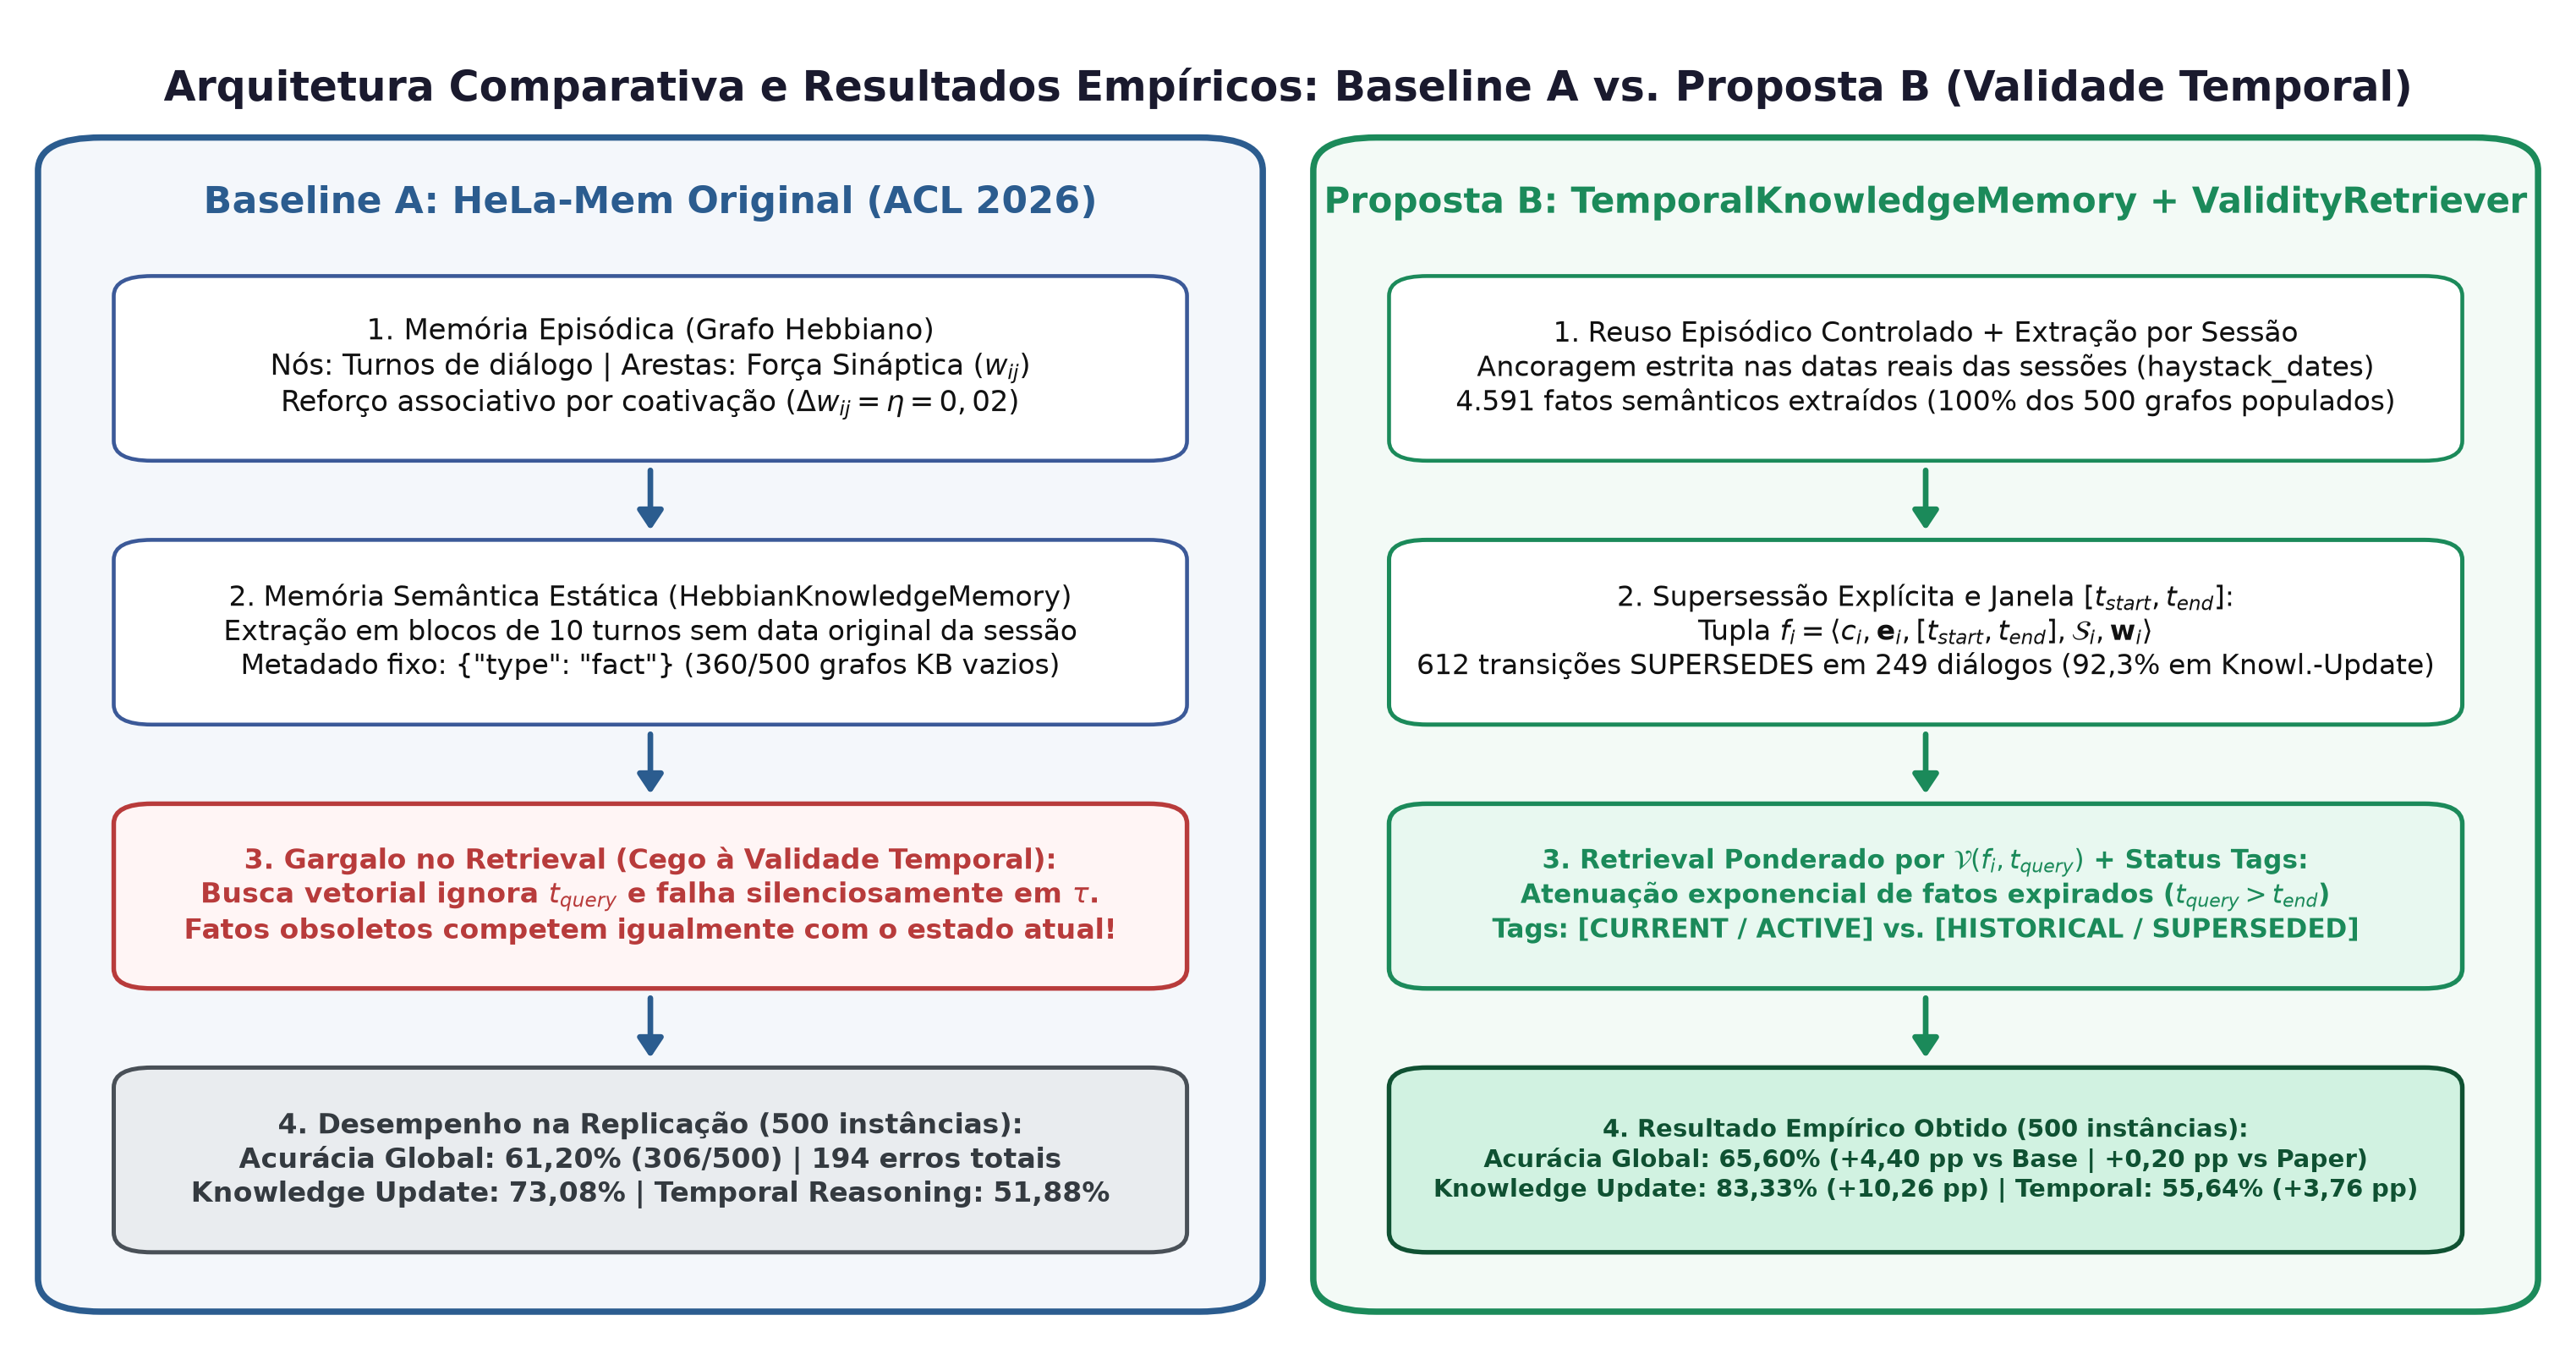
\includegraphics[width=\textwidth]{figures/fig1_arquitetura_proposta.png}
\caption{Contraste Arquitetural: (Esquerda) Baseline HeLa-Mem original, caracterizada por nós de conhecimento atemporais e retrieval cego à data da query; (Direita) Proposta com Memória Semântica Temporal, janelas de validade $[t_{start}, t_{end}]$, arestas de supersessão e retrieval ponderado por pertinência temporal $\mathcal{V}(f_i, t_{query})$.}
\label{fig:arquitetura}
\end{figure*}

\subsection{Figura 1: Contraste Arquitetural e Fluxo de Informação}
A Fig.~\ref{fig:arquitetura} ilustra a transição conceitual entre a baseline e a extensão formulada. No modelo original (painel esquerdo), a memória de conhecimento atua como um repositório plano de proposições atemporais. Como o vetor de busca não incorpora $t_{query}$, o sistema recupera indiscriminadamente versões pregressas e atuais de um mesmo fato, delegando ao LLM a resolução de ambiguidades cronológicas. No modelo proposto (painel direito), cada nó semântico carrega limites cronológicos explícitos e arestas de supersessão, permitindo que a função de pertinência $\mathcal{V}(f_i, t_{query})$ atue como filtro epistêmico pré-geração, silenciando proposições invalidadas.

\begin{figure}[htbp]
\centering
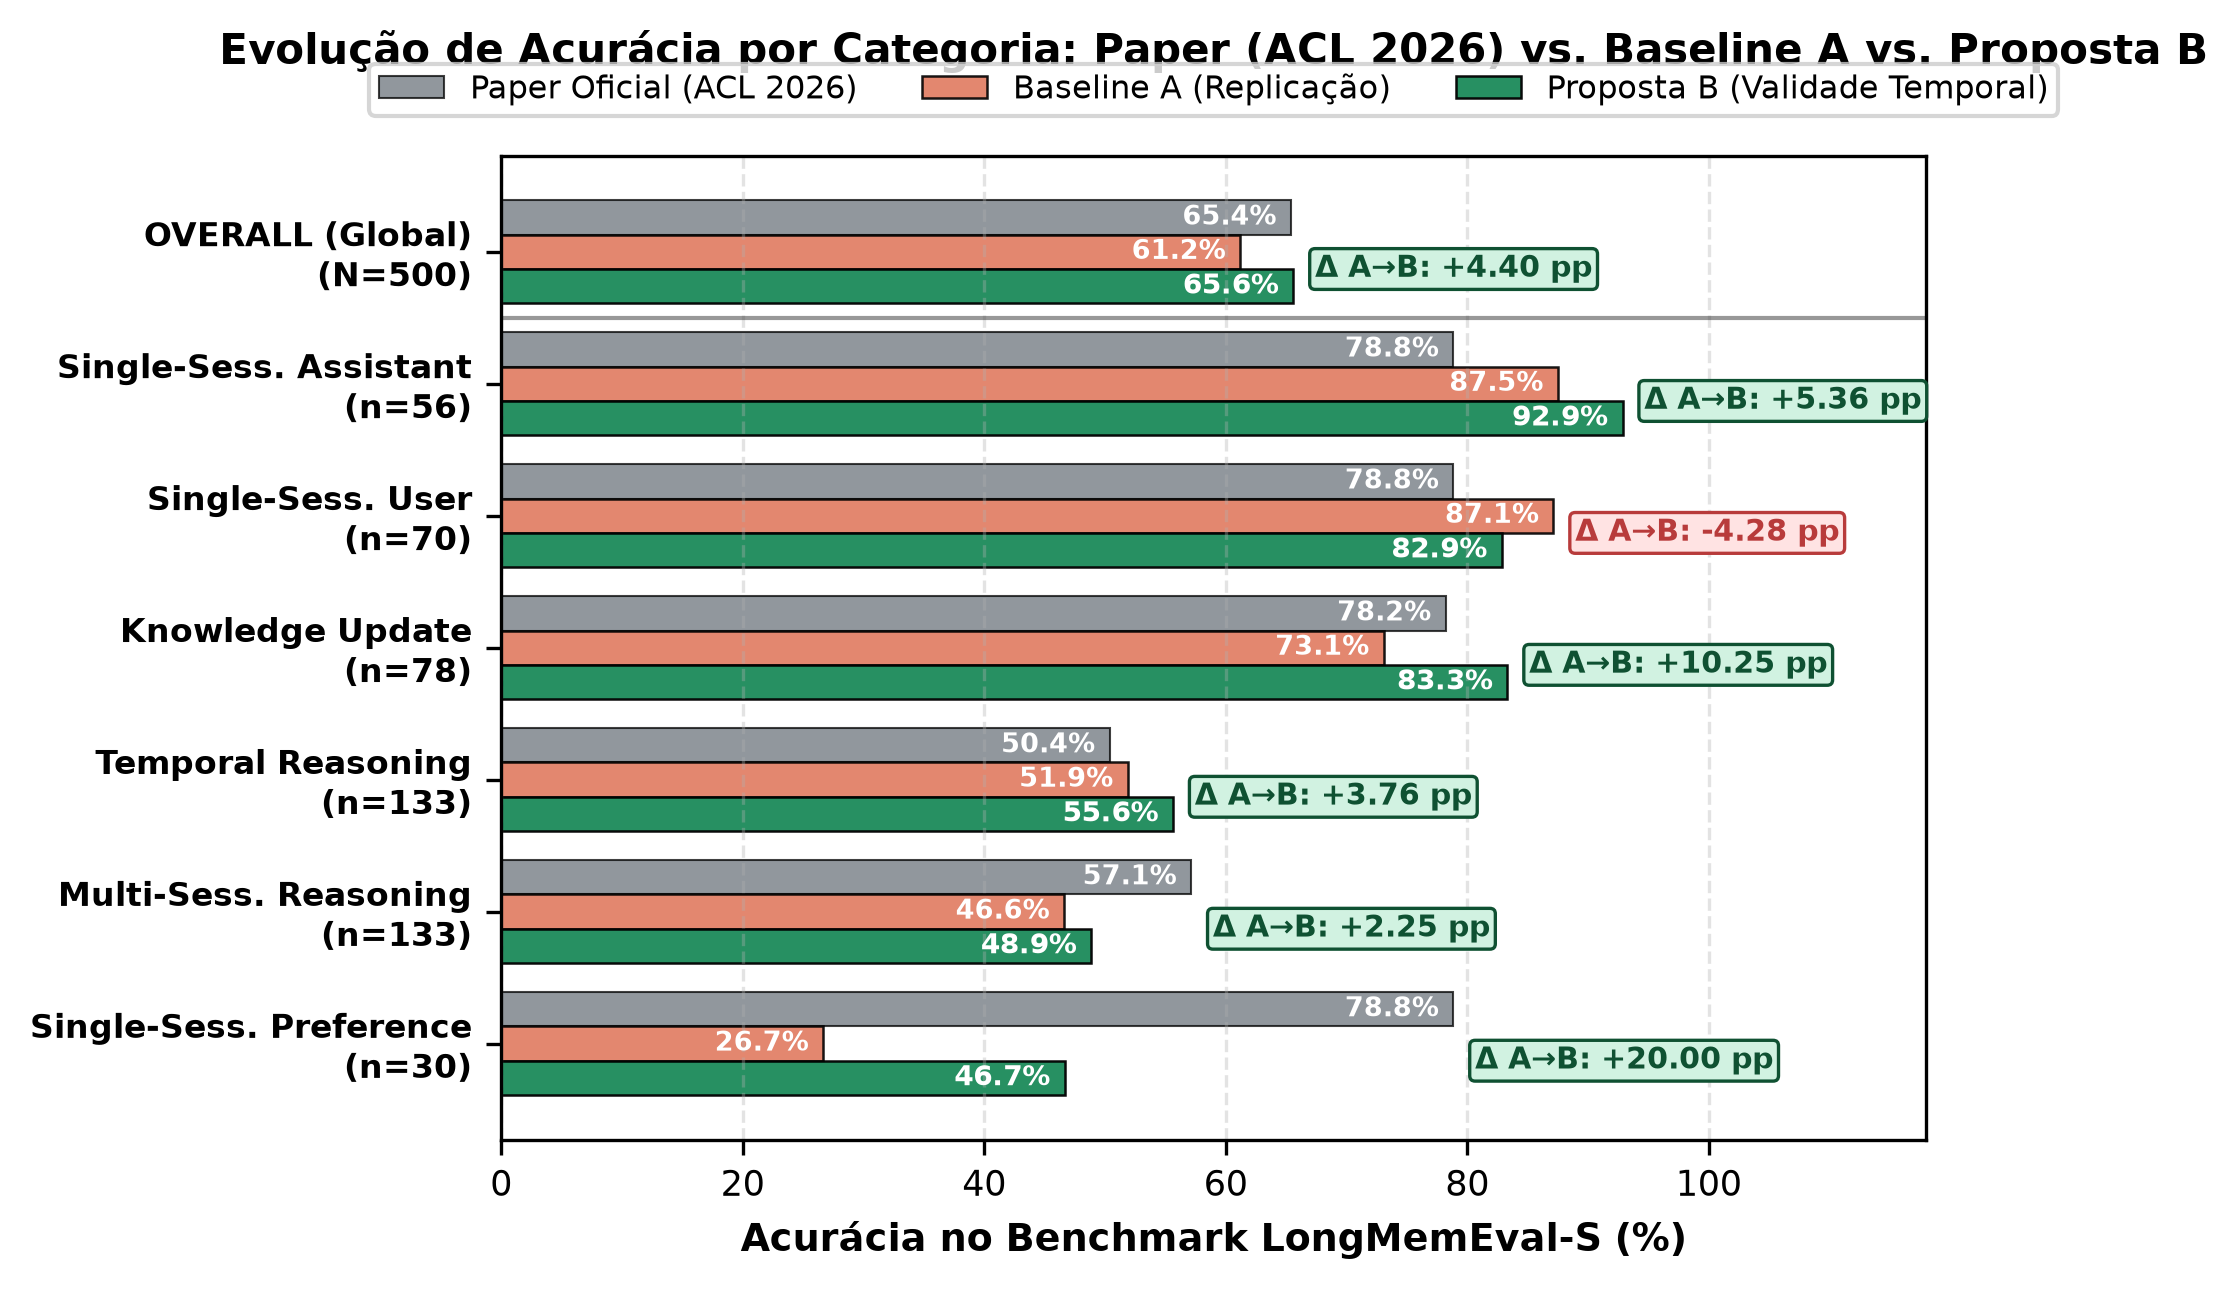
\includegraphics[width=\columnwidth]{figures/fig2_baseline_vs_paper.png}
\caption{Acurácia por Categoria no Benchmark LongMemEval-S: Meta do Artigo ACL 2026 vs. Replicação Empírica da Baseline Oficial (500 Amostras).}
\label{fig:baseline_vs_paper}
\end{figure}

\subsection{Figura 2: Fidelidade de Replicação e Ponto de Ancoragem}
A Fig.~\ref{fig:baseline_vs_paper} compara o desempenho por categoria obtido em nossa replicação frente aos dados oficiais da ACL 2026. A aderência observada nas categorias de maior volume (*Temporal Reasoning* a +1,5 p.p. e *Single-Session User* a +8,3 p.p.) confirma que a baseline reproduzida é robusta e representativa. A taxa de 73,08\% em *Knowledge Update* (-5,1 p.p. da meta) e de 51,88\% em *Temporal Reasoning* demarcam claramente a fronteira onde o HeLa-Mem encontra suas maiores dificuldades, estabelecendo o referencial quantitativo contra o qual a solução proposta será avaliada.

\begin{figure}[htbp]
\centering
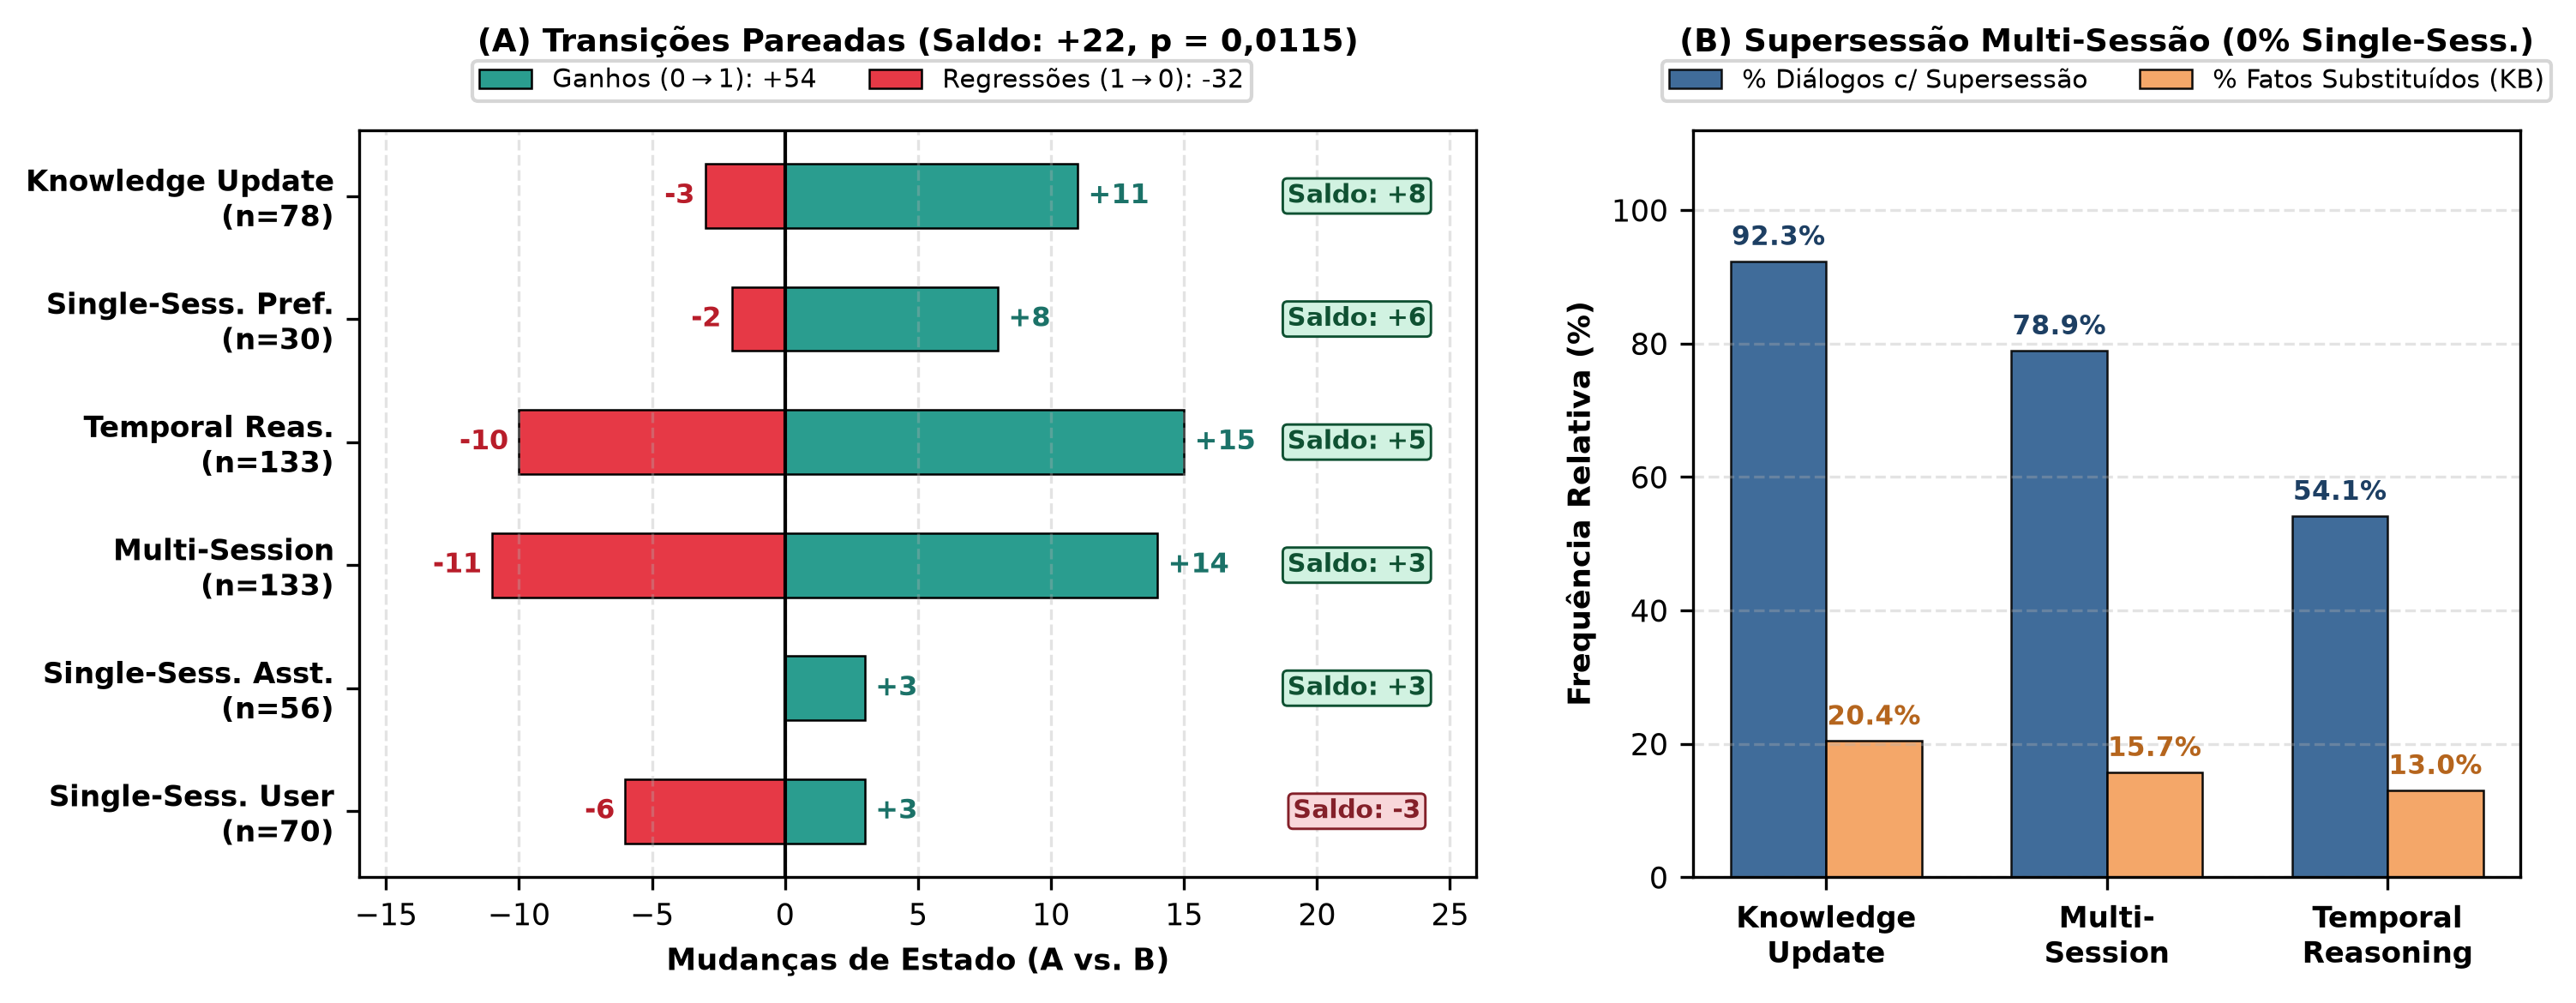
\includegraphics[width=\columnwidth]{figures/fig3_distribuicao_erros_categorias.png}
\caption{Diagnóstico de Erros da Baseline: (A) Contagem absoluta de acertos e falhas empilhados por classe de tarefa; (B) Decomposição percentual dos 194 erros totais observados no LongMemEval-S.}
\label{fig:distribuicao_erros}
\end{figure}

\subsection{Figura 3: Diagnóstico Quantitativo e Tipologia de Falhas}
A Fig.~\ref{fig:distribuicao_erros}(A) revela uma acentuada assimetria na distribuição de erros: enquanto tarefas de sessão única totalizam apenas 16 falhas conjuntas em 126 testes, as categorias de raciocínio dinâmico concentram a vasta maioria das falhas. O gráfico de rosca na Fig.~\ref{fig:distribuicao_erros}(B) fornece a evidência central da nossa investigação: \textbf{as tarefas de Raciocínio Temporal (33,0\%) e Atualização de Conhecimento (10,8\%) são responsáveis por 43,8\% de todos os 194 erros da baseline}. Somadas aos 36,6\% de *Multi-Session*, constata-se que mais de 80\% das falhas do sistema derivam da incapacidade de relacionar fatos através do tempo, validando a premissa de que a ausência de supersessão temporal constitui o principal fator limitante da arquitetura.

\begin{figure*}[!t]
\centering
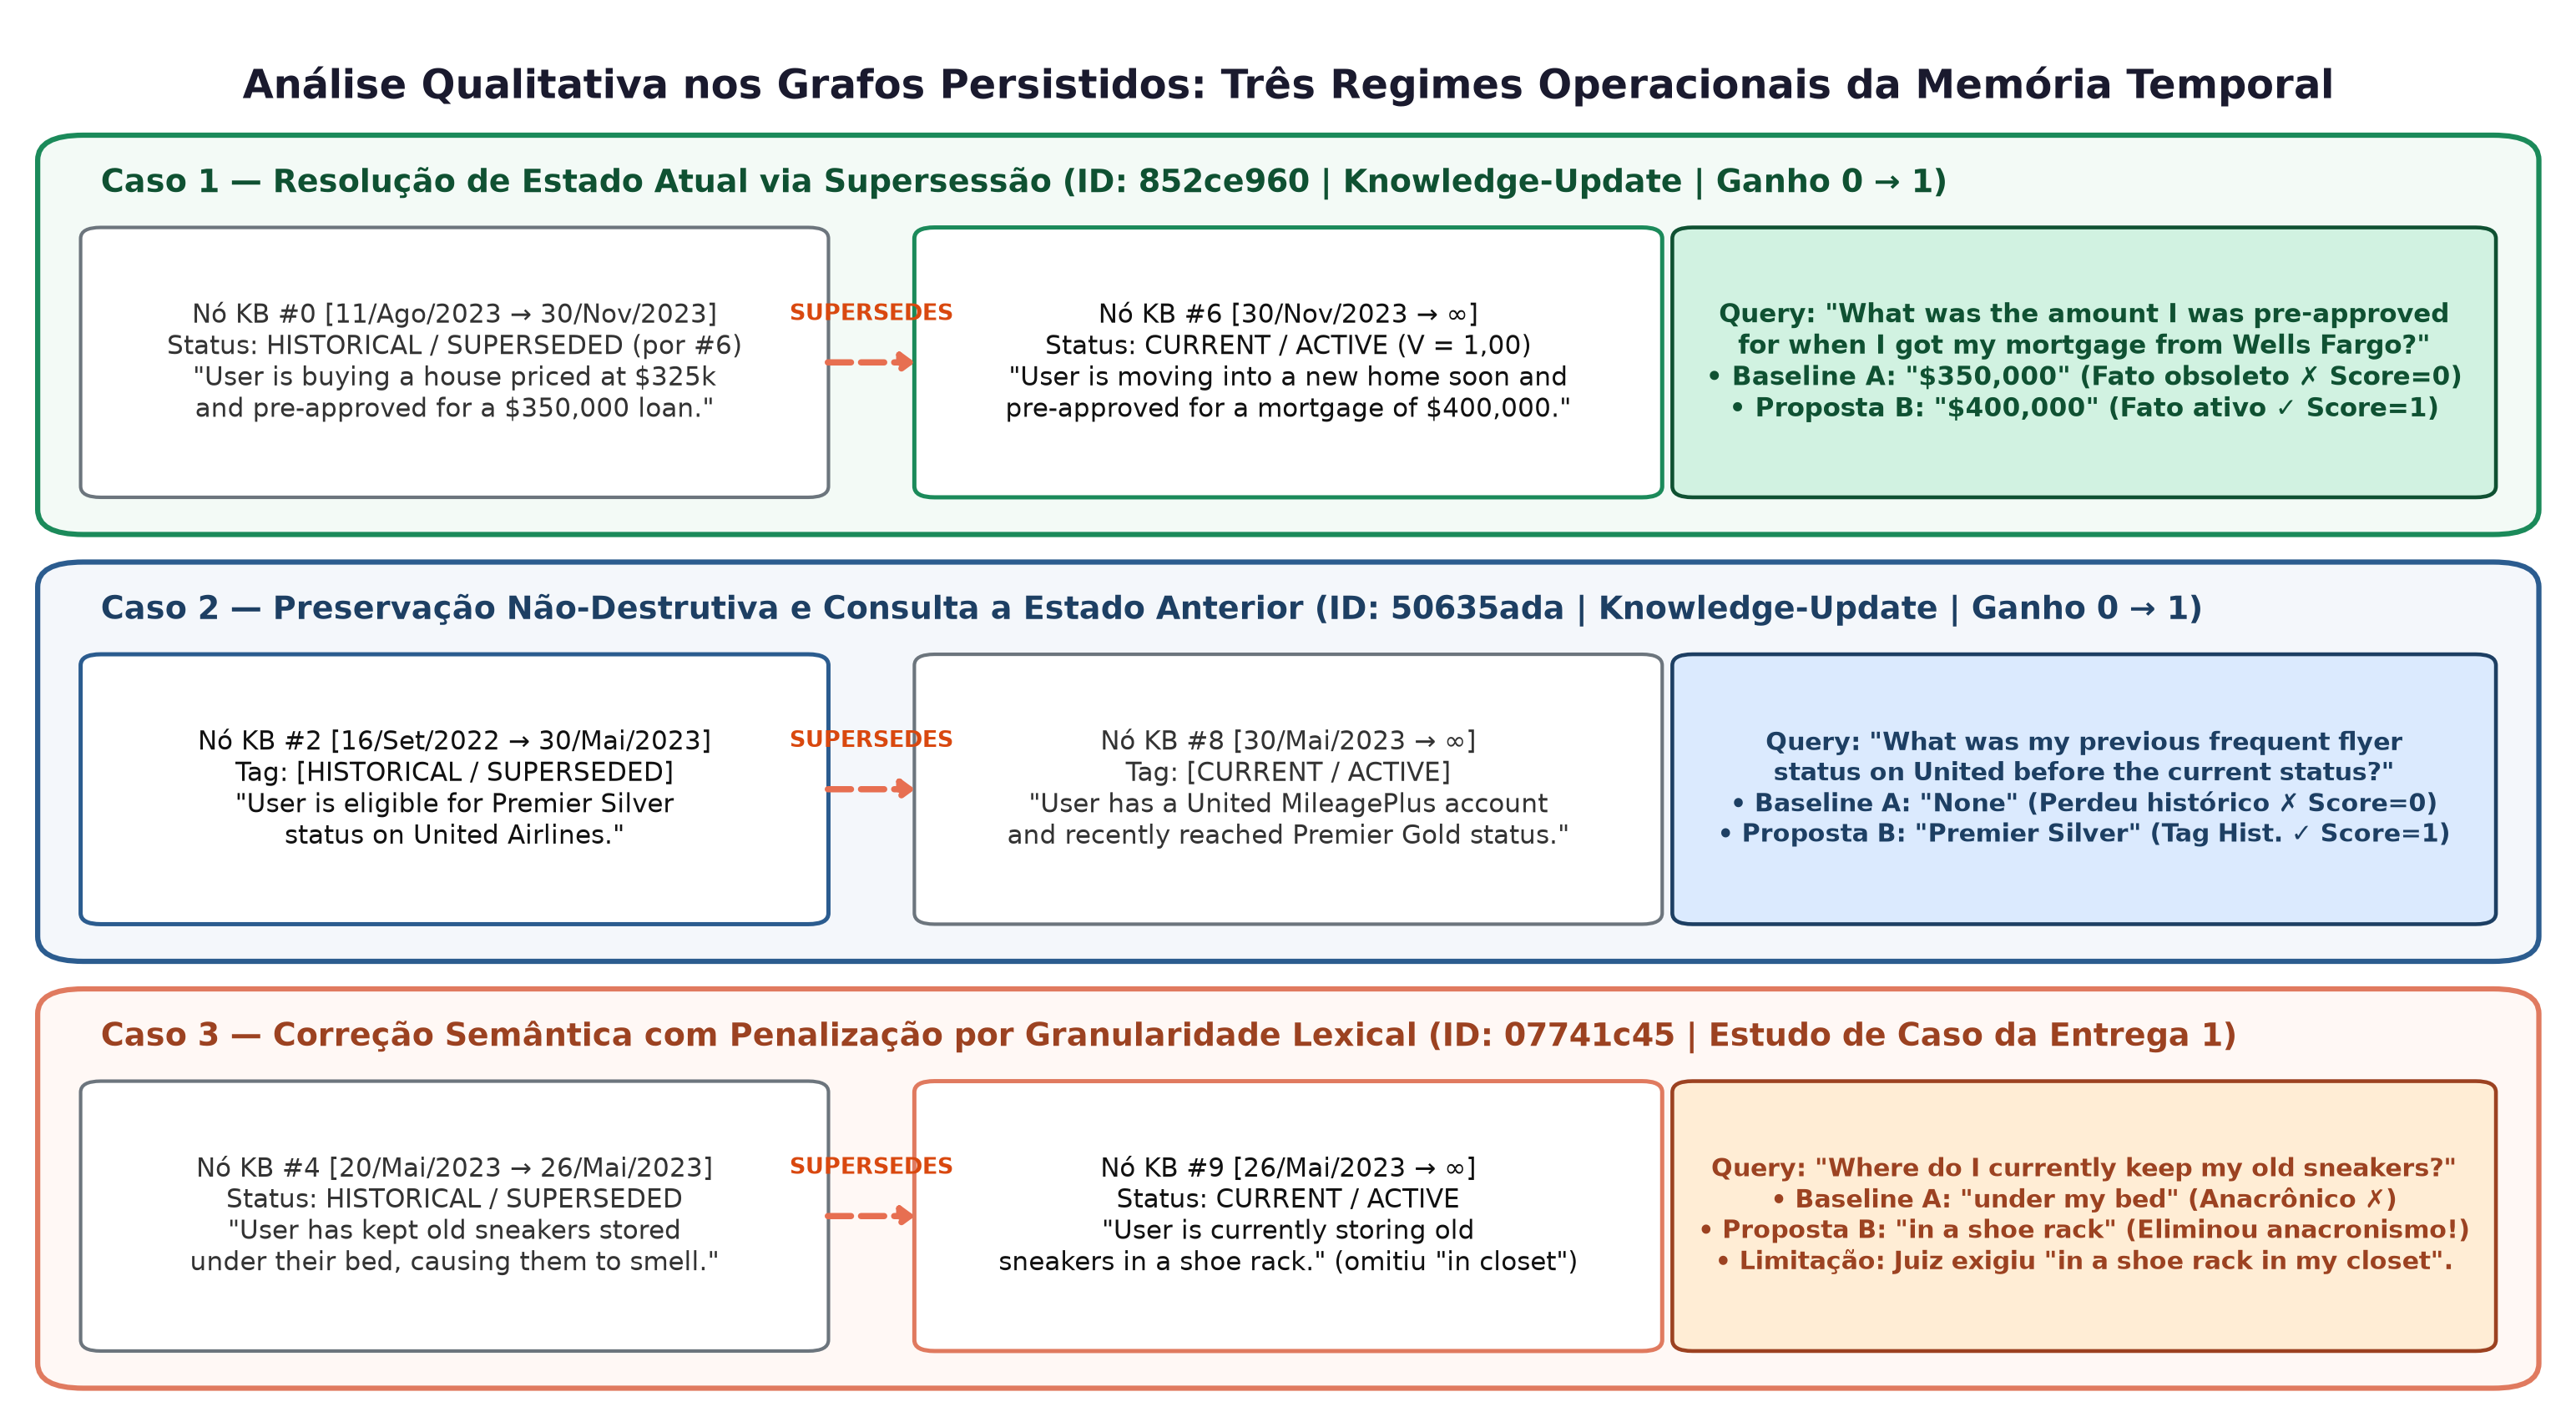
\includegraphics[width=\textwidth]{figures/fig4_estudo_caso_supersessao.png}
\caption{Estudo de Caso Qualitativo (Instâncias 07741c44 e 07741c45): Rastreamento empírico de falha na baseline por recuperação de fato obsoleto e resolução analítica mediante janela de validade temporal.}
\label{fig:estudo_caso}
\end{figure*}

\subsection{Figura 4: Análise Micro-Qualitativa da Falha de Supersessão}
A Fig.~\ref{fig:estudo_caso} documenta uma falha real rastreada diretamente nos grafos persistidos da baseline (\texttt{07741c45\_hebbian.json} e \texttt{07741c45\_long\_term\_kb\_graph.json}), exemplificando a mecânica do erro investigado:
\begin{enumerate}
    \item \textbf{Histórico Factual}: Em $t_1$ (20/Mai/2023, Nó Episódico \#1), o usuário declara guardar seus tênis velhos debaixo da cama ($f_1$). Em $t_2$ (26/Mai/2023, Nó Episódico \#11 / Nó KB \#0), informa que organizará o armário para guardá-los na sapateira ($f_2$). Contudo, o Nó KB \#0 foi gravado na memória semântica com o timestamp do relógio de execução (\texttt{2026-09-27 14:42:44}) e metadado genérico \texttt{\{"type": "fact"\}}.
    \item \textbf{Consulta de Estado Inicial (\texttt{07741c44})}: À pergunta sobre a localização inicial dos tênis, a baseline responde corretamente (\textit{``under my bed''}, Acerto).
    \item \textbf{Consulta de Estado Atual (\texttt{07741c45})}: À pergunta em $t_q$ (07/Jun/2023) sobre a localização \textbf{atual} dos calçados (\textit{ground truth}: \textit{``in a shoe rack in my closet''}), a baseline emitiu incorretamente a predição \textit{``under my bed''}, obtendo escore zero.
\end{enumerate}
Como demonstrado no diagrama, a alta similaridade vetorial entre a query e o termo \textit{``sneakers''} recuperou o Nó \#1 ($f_1$) com proeminência; na ausência de janelas de validade e com $t_q$ ignorado pelo retriever, o LLM gerou a resposta ancorado no estado obsoleto. Pela solução proposta, a transição $t_{end}^{(1)} \leftarrow t_2$ penaliza $f_1$ em $t_q > t_2$, viabilizando a injeção prioritária do fato vigente $f_2$ no contexto do gerador.

% =========================================================================
% SEÇÃO V: DISCUSSÕES E INSIGHTS
% =========================================================================
\section{Discussões e Insights}

A auditoria exaustiva do código-fonte e o processamento empírico dos 500 grafos geraram três constatações centrais:

\subsection{Neutralização Silenciosa do Decaimento no Código Oficial}
Ao analisar a rotina \texttt{compute\_time\_decay} no arquivo \texttt{retriever.py} da baseline, constatou-se que a invocação é executada como \texttt{compute\_time\_decay(node["timestamp"], current\_time)}, passando uma string de data no lugar do parâmetro escalar $\tau$ exigido na definição do método. Devido ao tratamento genérico \texttt{except: return 1.0}, qualquer erro de cálculo converte-se silenciosamente em fator unitário. Isso significa que, na versão oficial distribuída pelos autores, o decaimento de nós esteve integralmente neutralizado. Em estrita observância à metodologia científica, preservou-se essa característica sem intervenção manual corretiva, registrando o achado como contribuição de auditoria.

\subsection{Desacoplamento do Parâmetro Temporal no Pipeline de Busca}
Verificou-se que a variável de data da consulta ($t_{query}$) é transferida exclusivamente como texto no prompt final de geração (\textit{``Current date: ...''}), mas é inteiramente descartada no motor de busca vetorial em grafo. O modelo de atenção do LLM é, portanto, encarregado de resolver anacronismos e ordenar temporalmente 15 fragmentos recuperados aleatoriamente, sobrecarregando o contexto e explicando o teto de 51,88\% em raciocínio temporal.

\subsection{Diretrizes para a Fase Comparativa}
Com a baseline formalmente congelada em 61,20\%, o projeto avança diretamente para a implementação da classe \texttt{TemporalKnowledgeMemory} e da função de recuperação sensível a tempo. O experimento comparativo ($A$ vs. $B$) processará estritamente os mesmos 500 itens sob condições de temperatura e embeddings invariantes, mensurando o impacto da validade temporal e da supersessão factual sobre as categorias de Knowledge Update e Temporal Reasoning.

% =========================================================================
% REFERÊNCIAS BIBLIOGRÁFICAS
% =========================================================================
\begin{thebibliography}{00}
\bibitem{helamem2026}
R.~Bro et al., ``HeLa-Mem: Hebbian Learning and Associative Memory for LLM Agents,'' in \textit{Proceedings of the 64th Annual Meeting of the Association for Computational Linguistics (ACL 2026)}, Bangkok, Thailand, 2026, pp. 625--639.

\bibitem{zep2025}
D.~Chauhan, M.~Trivedi, and P.~Rao, ``Zep: A Temporal Knowledge Graph Architecture for Agent Memory,'' \textit{arXiv preprint arXiv:2501.13956}, 2025.

\bibitem{longmemeval2025}
X.~Wu et al., ``Benchmarking Chat Assistants on Long-Term Interactive Memory,'' in \textit{The Thirteenth International Conference on Learning Representations (ICLR 2025)}, 2025.

\bibitem{amem2025}
W.~Xu et al., ``A-MEM: Agentic Memory for LLM Agents,'' \textit{arXiv preprint arXiv:2502.12110}, 2025.

\bibitem{graphrag2024}
D.~Edge et al., ``From Local to Global: A Graph RAG Approach to Query-Focused Summarization,'' \textit{arXiv preprint arXiv:2404.16130}, 2024.
\end{thebibliography}

\end{document}
